\chapter{¿Qué es una simulación? Gazebo}
\label{cap:simulacion}

\begin{enpocas}
Por qué se simula antes de volar, qué hace un simulador de robots como Gazebo, cómo se describe un
robot (SDF), la diferencia entre lo que se ve y lo que choca, qué son los \emph{plugins} y qué
significan SITL y ``factor de tiempo real''.
\end{enpocas}

\section{¿Por qué simular?}

Un Tarot 650 con cámara cuesta varios miles de pesos y un error de programación puede estrellarlo en
segundos. Además, para probar la búsqueda de un incendio harían falta un bosque, un incendio y
permisos. Un simulador resuelve todo eso:
\begin{itemize}
  \item los choques son gratis: se reinicia y listo;
  \item se puede repetir exactamente el mismo experimento (mismo viento, mismo incendio) para comparar
        controladores, algo imposible al aire libre;
  \item se puede medir todo, incluida la posición \emph{verdadera} del dron, que en la vida real nunca
        se conoce exactamente;
  \item se puede acelerar o pausar el tiempo.
\end{itemize}
A cambio, un simulador es una aproximación: el viento, la aerodinámica o la cámara nunca son
idénticos a los reales. Por eso el camino es simular, luego volar con cuidado y comparar.

\begin{recuerda}
La simulación no reemplaza el vuelo real: lo prepara. Lo que no funciona en simulación, casi seguro
no funcionará en el dron; lo que funciona en simulación, probablemente funcionará con ajustes.
\end{recuerda}

\section{Gazebo}

\textbf{Gazebo} (en su versión \emph{Harmonic}) es un simulador de robots de código abierto. En cada
paso de tiempo (1~ms en nuestro caso):
\begin{enumerate}
  \item un \textbf{motor de física} (DART) calcula fuerzas, contactos y movimientos de todos los
        cuerpos, resolviendo ecuaciones como las del capítulo anterior;
  \item un \textbf{motor de render} (OGRE 2) dibuja la escena en 3D, lo que permite simular cámaras y
        LiDAR;
  \item los \textbf{sensores} simulados (IMU, cámara, LiDAR, odometría) generan sus mediciones;
  \item los \textbf{plugins} (pequeños programas) agregan comportamientos: motores, viento, partículas
        de fuego, conexión con ArduPilot.
\end{enumerate}

\begin{figure}[H]
\centering
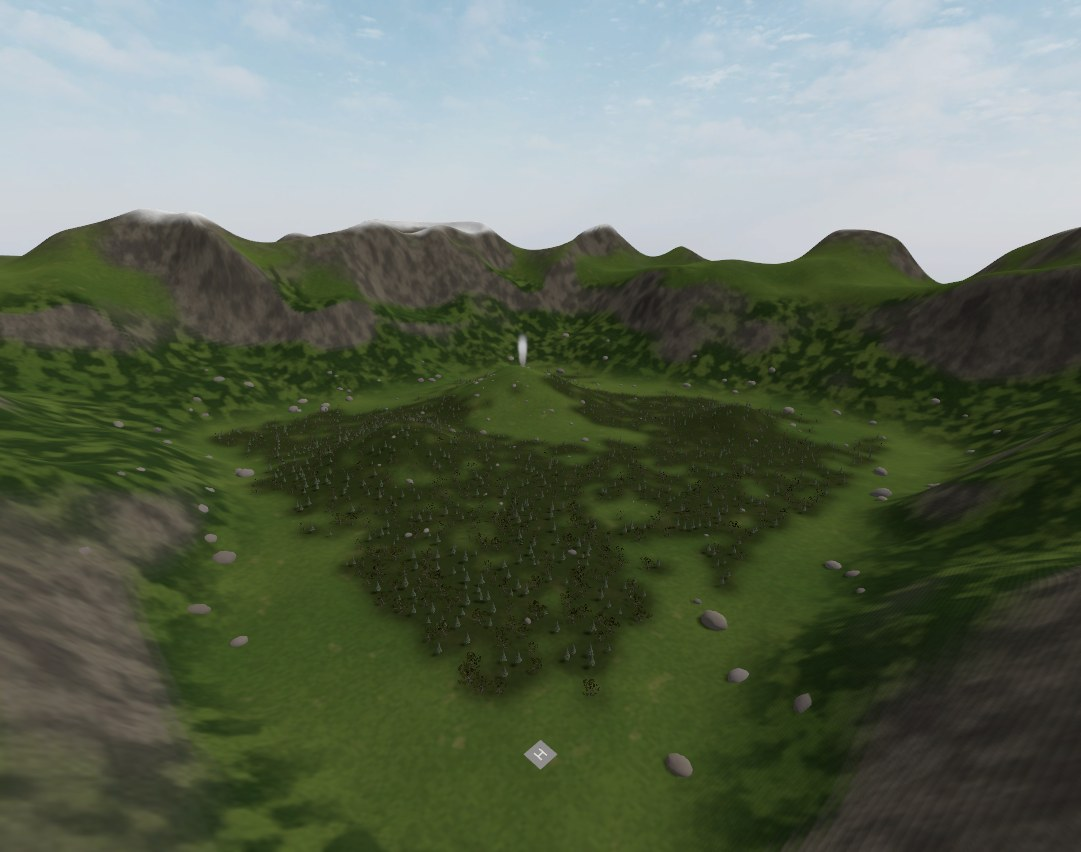
\includegraphics[width=\textwidth]{gz_valle_aereo.jpg}
\caption{El mundo \cod{bosque_grande} visto en Gazebo: terreno, árboles, rocas, cielo y, al fondo, el
humo del incendio.}
\end{figure}

\section{Cómo se describe un robot: SDF}

Gazebo lee los robots y los mundos en archivos \textbf{SDF} (\emph{Simulation Description Format}),
que son texto en formato XML. Un robot se describe con:
\begin{description}
  \item[Eslabones (\emph{links}):] piezas rígidas, cada una con masa, inercia, una forma para dibujar
        y otra para chocar. El Tarot tiene el cuerpo y cuatro rotores.
  \item[Articulaciones (\emph{joints}):] cómo se unen los eslabones; los rotores giran respecto al
        cuerpo en articulaciones \emph{revolute}.
  \item[Sensores] montados en un eslabón, con su posición y orientación.
  \item[Plugins] que les dan vida.
\end{description}

Un fragmento simplificado:
\begin{lstlisting}[style=xml]
<model name="cuadrirotor">
  <link name="base_link">
    <inertial><mass>2.12</mass> ... </inertial>
    <visual name="placas"> <geometry><mesh><uri>model://tarot650/meshes/placas.stl</uri></mesh></geometry> </visual>
    <collision name="cuerpo_col"> <geometry><box><size>0.16 0.16 0.06</size></box></geometry> </collision>
    <sensor name="camara" type="camera"> ... </sensor>
  </link>
  <link name="rotor_0"> ... </link>
  <joint name="rotor_0_joint" type="revolute"> <parent>base_link</parent> <child>rotor_0</child> ... </joint>
  <plugin filename="gz-sim-multicopter-motor-model-system" ...> ... </plugin>
</model>
\end{lstlisting}

\section{Lo que se ve y lo que choca}

Cada eslabón tiene dos formas. La \textbf{visual} es la que se dibuja: puede ser una malla 3D muy
detallada, como la del CAD del Tarot. La de \textbf{colisión} es la que usa la física para detectar
choques: conviene que sea simple (cajas, cilindros) porque calcular contactos entre mallas
complicadas es lento y frágil.

\begin{figure}[H]
\centering
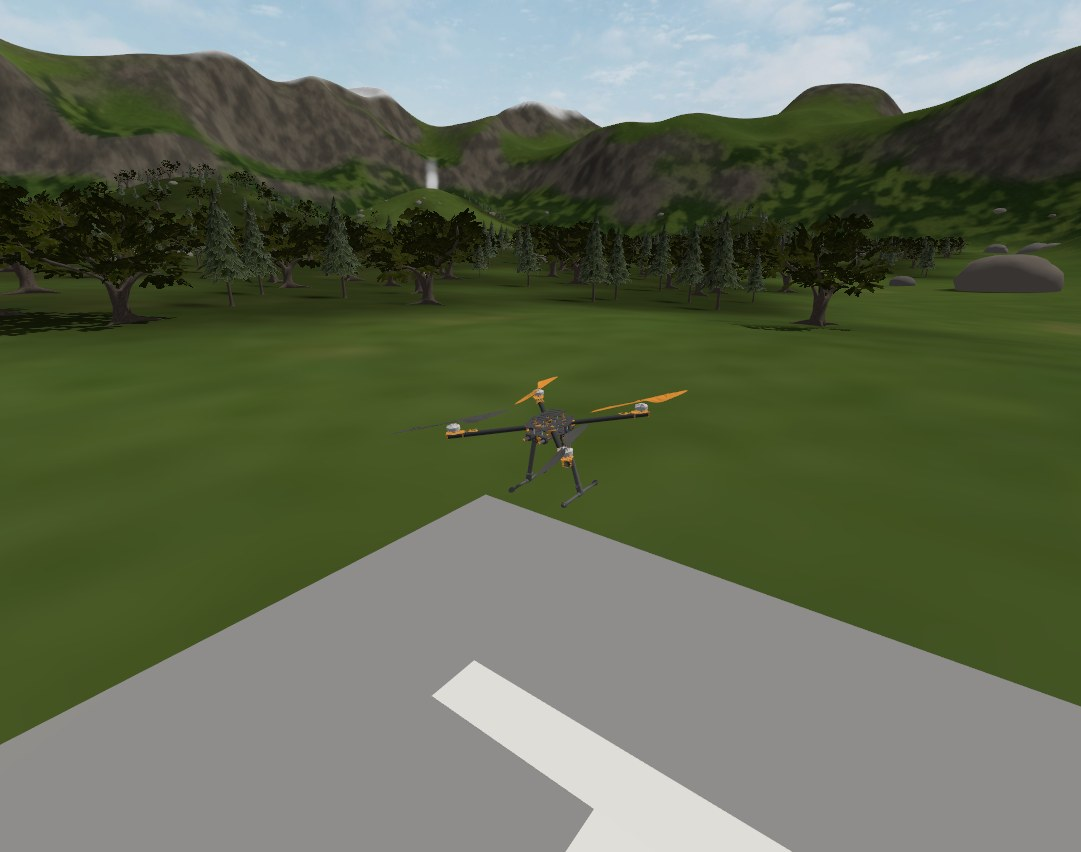
\includegraphics[width=0.48\textwidth]{gz_tarot_cerca.jpg}\hfill
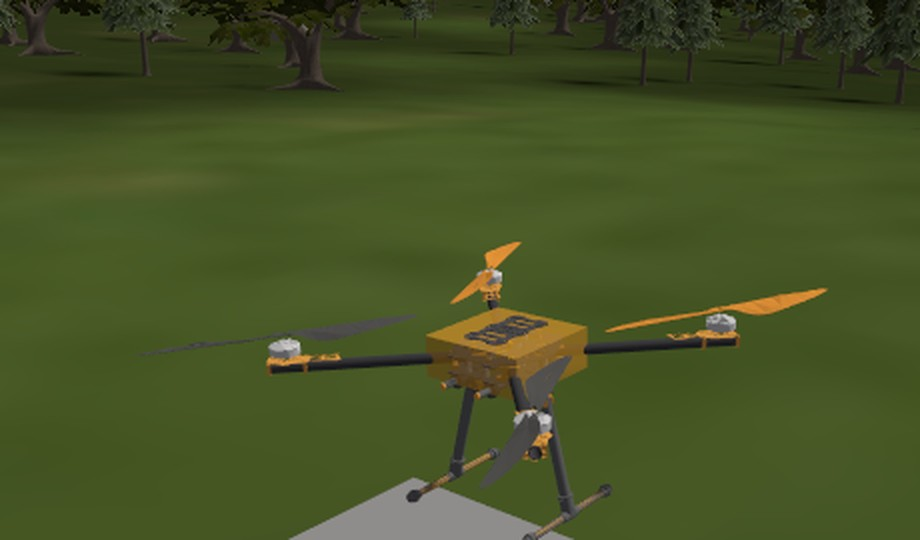
\includegraphics[width=0.48\textwidth]{gz_tarot_colisiones.jpg}
\caption{Izquierda: la forma visual del Tarot. Derecha: Gazebo mostrando sus formas de colisión (en
naranja): una caja para el cuerpo y dos cilindros delgados para los patines.}
\end{figure}

\begin{leccion}
En el mundo grande, las rocas usaban como colisión mallas OBJ sin \emph{normales} (los vectores que
dicen hacia dónde ``mira'' cada triángulo). Gazebo se caía con un \emph{segfault} en cuanto algo las
tocaba. Exportarlas con normales lo arregló.
\end{leccion}

\section{Plugins}

Un \emph{plugin} es código (en C++) que Gazebo carga para agregar un comportamiento. En este proyecto
se usan:
\begin{description}
  \item[\cod{MulticopterMotorModel}] (de Gazebo): convierte una velocidad pedida en empuje y par de un
        rotor, con su retardo.
  \item[\cod{OdometryPublisher}:] publica la posición y velocidad verdaderas del dron.
  \item[\cod{ParticleEmitter}:] las llamas y el humo.
  \item[\cod{FuerzaViento}] (nuestro): aplica la fuerza del viento.
  \item[\cod{ComandosMotores}] (nuestro) y \cod{ArduPilotPlugin}: para volar con ArduPilot.
\end{description}

\section{Tiempo simulado y factor de tiempo real}

La simulación tiene su propio reloj. Si la computadora es rápida, un segundo simulado tarda un segundo
real; si no, tarda más. El \textbf{factor de tiempo real} (RTF) es la razón entre los dos: RTF = 1
significa tiempo real; RTF = 0.5, que todo va a la mitad de velocidad. Con la RTX 5060 Ti el mundo
grande corre a RTF $\approx$1.0 (0.8 con el LiDAR). Todos los nodos usan el reloj simulado
(\cod{use_sim_time}), así que los resultados no dependen de la velocidad de la computadora.

\section{SITL y HITL}

\begin{description}
  \item[SITL] (\emph{software in the loop}): el mismo programa del piloto automático que volaría en el
        dron (aquí ArduCopter) corre en la computadora y ``vuela'' el dron simulado. Es lo que hacemos
        en el capítulo~\ref{cap:autopiloto}.
  \item[HITL] (\emph{hardware in the loop}): el controlador de vuelo físico está conectado a la
        simulación. Es el paso siguiente antes de volar.
\end{description}

\begin{ejercicio}
Lanza la simulación (capítulo~\ref{cap:primer-vuelo}) y, en la ventana de Gazebo, haz clic derecho
sobre el dron $\rightarrow$ \emph{View} $\rightarrow$ \emph{Collisions}. Verás las formas de choque.
Prueba también \emph{Inertia} y \emph{Frames}.
\end{ejercicio}
